%%%%%%%%%%%%%%%%%%%%%%%%% preamble %%%%%%%%%%%%%%%%%%
\documentclass{article}
\usepackage[utf8]{inputenc}  % input encoding
\usepackage{graphicx}  % to insert figures
\usepackage{amsmath,amsfonts}  %to insert complex equations

\usepackage{natbib}  % bibliography package
\bibliographystyle{dinat}  % bibliography style

\usepackage{hyperref}  %

\usepackage[english]{babel}  % to insert text in English
\usepackage{blindtext}  % to insert sample text



\title{Intro to \LaTeX}
\author{Dr Patricia Ternes\thanks{p.ternesdallagnollo@leeds.ac.uk}}
\date{\today}
%%%%%%%%%%%%%%%%%%%%%%%%% preamble %%%%%%%%%%%%%%%%%%


\begin{document}
\maketitle
\begin{abstract}
    \blindtext[1]
\end{abstract}

\tableofcontents
\listoftables
\listoffigures

%%%%%%%%%%%%%%%%%%%%%%%%% sessions and subsections! %%%%%%%%%%%%%%%%%%
\section{Introduction}
\blindtext[1]
\subsection{My first subsection}
\blindtext[1]
\subsection{Another subsection}
\blindtext[1]
\subsection{Another subsection}
\blindtext[1]
\subsubsection{Sub sub session}
\blindtext[1]
\paragraph{Is it works?}
\blindtext[1]

%%%%%%%%%%%%%%%%%%%%%%%%% Lists! %%%%%%%%%%%%%%%%%%
\section{Lists}
\subsection{Unordered List}
\begin{itemize}
    \item red
    \item blue
    \item green
\end{itemize}

\blindtext[1]

\subsection{Description List}
\begin{description}
    \item[apple] red
    \item[sky] blue
    \item[leaf] green
    \item yellow
\end{description}

\blindtext[1]

\subsection{Ordered List}
\begin{enumerate}
    \item green
    \item red
    \item yellow
    \item blue
\end{enumerate}

\blindtext[1]

\subsection{Nested list}
\begin{enumerate}
    \item green
    \begin{itemize}
        \item leaf
    \end{itemize}
    \item red
    \begin{itemize}
        \item apple
    \end{itemize}
    \item yellow
    \item blue
\end{enumerate}


%%%%%%%%%%%%%%%%%%%%%%%%% Figures! %%%%%%%%%%%%%%%%%%
\section{Figure}\label{sec:fig}
Figure \ref{fig:sample-fig} shows a sample figure from the graficx package.
\blindtext[1]
\begin{figure}[h]
    \centering
    \includegraphics[width=0.4\textwidth]{example-grid-100x100bp}
    \caption{Sample figure from graphicx package.}
    \label{fig:sample-fig}  % used to reference the figure in the text
\end{figure}

Figure \ref{fig:uni-pic} shows a picture of University of Leeds. This picture is part of the Session \ref{sec:fig}.
\blindtext[1]
\begin{figure}[h]  % [h] = try to put float "here"
    \centering
    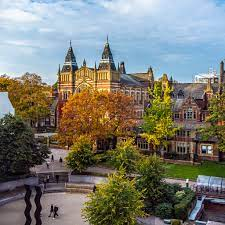
\includegraphics[width=0.4\textwidth]{uni.jpg}
    \caption{University of Leeds picture.}
    \label{fig:uni-pic}  % used to reference the figure in the text
\end{figure}


%%%%%%%%%%%%%%%%%%%%%%%%% Table! %%%%%%%%%%%%%%%%%%
\section{Table}\label{sec:tab}
\blindtext[1] See Table \ref{tab:col_fruit} in Session \ref{sec:tab} to see a fruit of each colour.
\begin{table}[h]
    \centering
    \begin{tabular}{|c||c|}\hline  % "\hline" = drawn a horizontal line
        Colour & Fruit     \\ \hline \hline % "&" = change column, "\\" = line break
        Red    & Apple     \\  
        Yellow & Banana    \\
        Green  & Grape     \\
        Blue   & blueberry \\ \hline
    \end{tabular}
    \caption{Table of colours and fruits.}
    \label{tab:col_fruit}
\end{table}

\blindtext[1]


%%%%%%%%%%%%%%%%%%%%%%%%% Math! %%%%%%%%%%%%%%%%%%
\section{Math}\label{sec:math}
You can insert math inline by using \$ delimiters, like: $y = \alpha + \beta x$.

You can add the equation in a new paragraph:
\[
\text{May the } \frac{d p}{d t} \text{ be with you!}
\]

Or you can add the equation in an ordered math environment:

According \cite{newton1850}, the force is defined as:
\begin{equation}
    F = ma = m\frac{dv}{dt} = \frac{dp}{dt},
\end{equation}
where $p$ is the momentum.

It is also possible combine the equation environment with an array environment:
\begin{equation}
    A = \left(
        \begin{array}{ccc}
            a_{11} & a_{12} & a_{13} \\
            a_{21} & a_{22} & a_{23} \\
            a_{31} & a_{32} & a_{33} \\
        \end{array}
    \right)
\end{equation}

\bibliography{sample}

\end{document}